\section{Practical examples and their caveats}
\frame{\tableofcontents[currentsection]}

\begin{frame}
    \frametitle{Basic load balancing with Nginx}
    \begin{center}
        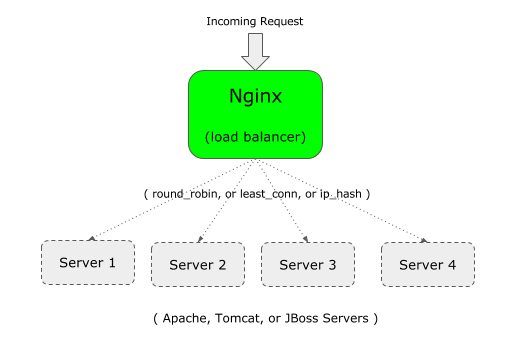
\includegraphics[scale=0.5]{01-nginx-basic.png}
    \end{center}
    \footnote{image from https://www.thegeekstuff.com/2017/01/nginx-loadbalancer/}
\end{frame}

\begin{frame}
    \frametitle{Downsides}
    \begin{itemize}
        \item no interaction between servers
        \item have to rely on external services
        \begin{itemize}
            \item X is running, how does other service/server know this? \\ 
            (DB) 
            \item queueing of jobs can't be coordinated between servers. \\ 
            (Redis)
            \item parallelization of a single server is hard to implement. \\ 
            (Nginx has no knowledge of the workload of a single server)
        \end{itemize}
    \item 1 http request is not equivalent to workload of 1 request
    \end{itemize}
\end{frame}



\begin{frame}
    \frametitle{Basic load balancing with Nginx}
    \begin{center}
        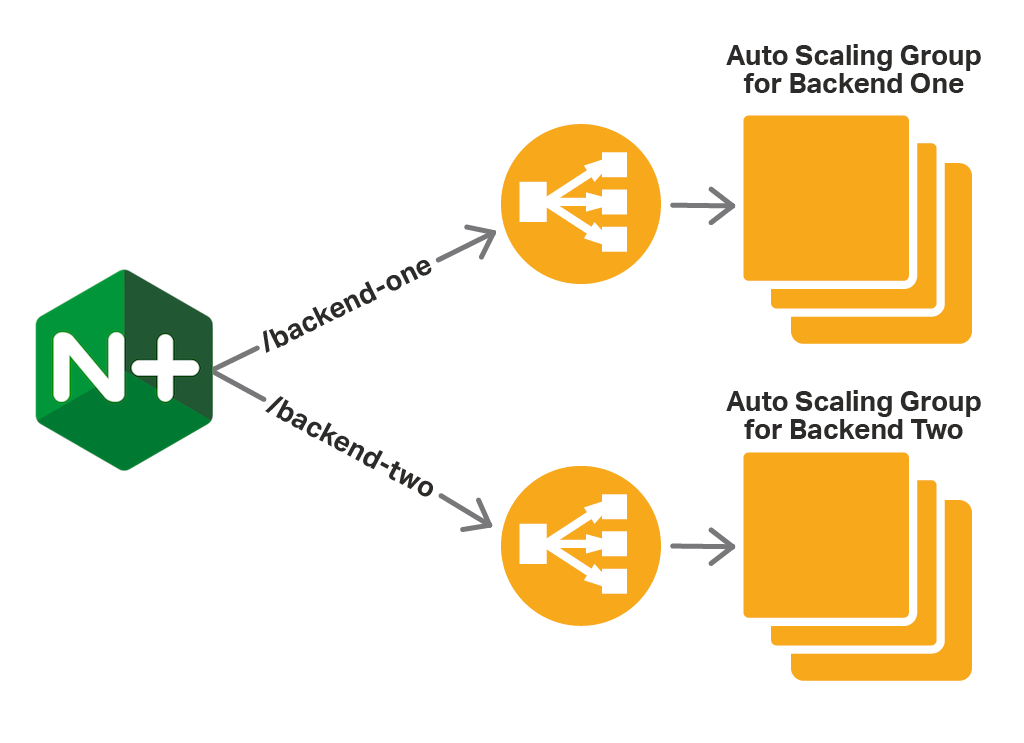
\includegraphics[scale=0.23]{02-nginx-aws-auto-scaling.png}
    \end{center}
    \footnote{image from https://www.nginx.com/blog/load-balancing-aws-auto-scaling-groups-nginx-plus/}
\end{frame}

\begin{frame}
    \frametitle{Downsides}
    \begin{itemize}
        \item has to pass through multiple load balancers
        \item previous problem(s) just minified
        \item Can be problematic for some use cases \\ 
        (unauthenticated user goes directly to secure route)
    \end{itemize}
\end{frame}



\begin{frame}
    \frametitle{Example of node groups in Erlang}
    \begin{center}
        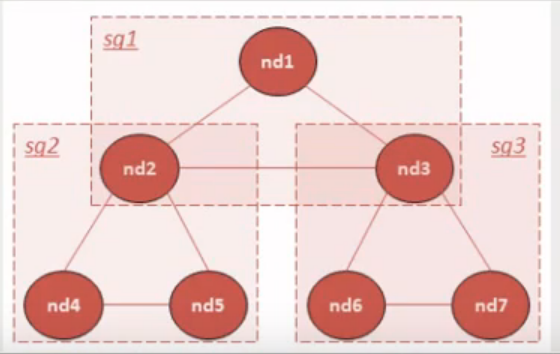
\includegraphics[scale=0.5]{03-sd-erlang.png}
    \end{center}
    \footnote{image from http://www.dcs.gla.ac.uk/research/sd-erlang/demos.html}
\end{frame}

\begin{frame}
    \frametitle{Downsides}
    \begin{itemize}
        \item complex setup
    \end{itemize}
\end{frame}